\documentclass{article}
\usepackage[a4paper, left=2.5cm, right=2.5cm, top=3cm,bottom=3cm]{geometry}
\usepackage[T1]{fontenc}
\usepackage[utf8]{inputenc}
% \usepackage{todonotes}
% \presetkeys{todonotes}{inline}{}

\usepackage[square, numbers, comma, sort&compress]{natbib}
\renewcommand\refname{References} % Adding title to referece section

\usepackage{xr-hyper} % For cross-referencing between the main article and supporting information
\usepackage[hidelinks]{hyperref}
\usepackage{stackengine} %Stacking symbols
\usepackage[version=4]{mhchem} %chemical equations

\usepackage{siunitx} %get SI units
\DeclareSIUnit{\atm}{atm}
\DeclareSIUnit{\angstrom}{\AA}
\DeclareSIUnit\bar{bar}

\renewcommand{\thefootnote}{\roman{footnote}} % Footnotes using roman numerals

\usepackage{float} %stuff that floats around
% \usepackage{dblfloatfix}    % To enable figure* floats at the bottom of page (figure must be declared before the page on which it should appear)
\usepackage{multirow}
\usepackage{booktabs}  %tables and stuff
\usepackage{tabularx}
\newcolumntype{Y}{>{\centering\arraybackslash}X} % To make tabularx spread the content across the column
\AtBeginDocument{% workaround for \toprule, \midrule and \bottomrule for revtex documentclass
  \heavyrulewidth=.08em
  \lightrulewidth=.05em
  \cmidrulewidth=.03em
  \belowrulesep=.65ex
  \belowbottomsep=0pt
  \aboverulesep=.4ex
  \abovetopsep=0pt
  \cmidrulesep=\doublerulesep
  \cmidrulekern=.5em
  \defaultaddspace=.5em
}


\usepackage{graphicx} %extra options when inputting figures
\usepackage[caption=false]{subfig} %subfigures
\usepackage{afterpage}

\usepackage{enumitem} % for listing stuff (bulletpoints and so on)
\usepackage{setspace} %if you want to change linespacing
\usepackage[parfill]{parskip} %spacing between paragraphs

\usepackage{amsmath, amssymb}
\usepackage{MnSymbol}
\usepackage{mathrsfs} % Nice, curly caligraphic with \mathscr
\usepackage{textgreek}
%Putting self-defined commands here

\renewcommand{\Vec}[1]{\boldsymbol{\mathrm{#1}}} % pretty vectors
\renewcommand{\vec}[1]{\Vec{#1}}
\newcommand{\Mat}[1]{\underline{\pmb{#1}}} % Matrices

% Common symbols
% Fluxes
\newcommand{\bvec}[1]{\Bar{\Vec{#1}}}
\newcommand{\flux}[2]{\Vec{J}_{#1}^{(#2)}}
\newcommand{\mflux}{\Vec{J}^{(n,m)}}
\newcommand{\qflux}{\Vec{J}_q}

% Thermo
% Vectors
\newcommand{\vx}{\vec{x}}
\newcommand{\vn}{\vec{n}}

\newcommand{\Lmm}{L_{\mu \mu}}
\newcommand{\Lmq}{L_{\mu q}}
\newcommand{\Lqm}{L_{q \mu}}
\newcommand{\Lqq}{L_{qq}}

\newcommand{\ST}{S_{T,1}}
\newcommand{\Kr}{K_{\rho}}
\newcommand{\Arho}{A_{\rho}}
\newcommand{\Brho}{B_{\rho}}

\newcommand{\Ta}{T^{\alpha}}
\newcommand{\Tb}{T^{\beta}}
\newcommand{\Va}{V^{\alpha}}
\newcommand{\Vb}{V^{\beta}}
\newcommand{\na}{n^{\alpha}}
\newcommand{\nb}{n^{\beta}}
\newcommand{\xa}{x^{\alpha}}
\newcommand{\xb}{x^{\beta}}
\newcommand{\vna}{\vn^{\alpha}}
\newcommand{\vnb}{\vn^{\beta}}
\newcommand{\vxa}{\vx^{\alpha}}
\newcommand{\vxb}{\vx^{\beta}}


% Kinetic gas theory
\newcommand{\vr}{\vec{r}}
\newcommand{\vu}{\vec{u}}
\newcommand{\bvu}{\Bar{\vec{u}}}
\newcommand{\cvel}[1]{\bvec{u}_{#1}}
\newcommand{\vU}{\vec{U}}
\newcommand{\cVel}{\bvec{U}}
\newcommand{\sD}{\mathscr{D}}
\newcommand{\sU}{\mathscr{U}}
\newcommand{\vsU}{\pmb{\mathscr{U}}}
\newcommand{\vA}{\vec{\Lambda}}
\newcommand{\tvA}{\Tilde{\vA}}
\newcommand{\vD}{\vec{D}}
\newcommand{\vd}{\vec{d}}
\newcommand{\mB}{\Mat{B}}
\newcommand{\va}{\vec{a}}
\newcommand{\sg}{\mathcal{g}}
\renewcommand{\d}{\mathrm{d}}
\newcommand{\rdf}{\Tilde{\chi}}

% Differentials
\renewcommand{\d}{\mathrm{d}}
\newcommand{\dT}{\d T}
\newcommand{\dV}{\d V}
\newcommand{\drho}{\d \rho}
\newcommand{\dr}{\d r}
\newcommand{\dn}{\d n}
\newcommand{\dx}{\d x}
\newcommand{\dA}{\d A}
\newcommand{\dmu}{\d\mu}

% Finite differences
\newcommand{\Dn}{\Delta n}
\newcommand{\Dx}{\Delta x}
\newcommand{\DT}{\Delta T}

\newcommand{\symbline}[3]{$ #1 $ & #2 & \si{#3} \\} % quick symbol table: \symbline{symbol}{description}{unit}
\newcommand{\abrline}[2]{#1 & #2 \\} % Abbreviation & Description
\newcommand{\subline}[2]{$#1$ & #2} % Subscript & Description
%%%%%%%%%%%%%%%%%%%%%%%%%%%%%%%%%%%%%%%%%%%%%%%%%%%%%%%%%%%%%%%%%%%%%%%%%%%%%%%%%%%%%%%%%%%%%%%%%%%%%%%%%%%%
%       quick maffs       %
\newcommand{\del}{\partial} 
\newcommand{\pfrac}[2]{\left(\frac{#1}{#2}\right)} %fraction with parentheses around
\newcommand{\pder}[2]{\frac{\del #1}{\del #2}} %partial derivative of x with respect to y as \pder{x}{y}
\newcommand{\ppder}[2]{\left(\pder{#1}{#2}\right)} %\pder{}{} but with parentheses
\newcommand{\der}[2]{\pfrac{\d #1}{\d #2}}
\newcommand{\lrp}{\left(}
\newcommand{\rrp}{\right)}
\newcommand{\lsp}{\left[}
\newcommand{\rsp}{\right]}
\newcommand{\lcp}{\left\{}
\newcommand{\rcp}{\right\}}
\newcommand{\DeltaAB}{\underset{\alpha,\beta}{\Delta}}
\newcommand{\DeltaIG}{\underset{ig}{\Delta}}
\newcommand{\DeltaHS}{\underset{HS}{\Delta}}
\newcommand{\stackmax}[1]{\stackanchor{$\max$}{\tiny{$#1$}}}

\newcommand{\spder}[3]{
  \ifthenelse{\equal{\detokenize{#2}}{\detokenize{#3}}}
    {\left(\frac{\del^2 #1}{\del #2^2}\right)}
    {\left(\frac{\del^2 #1}{\del #2 \del #3}\right)}%
}

\newcommand{\abs}[1]{\left|#1\right|}
\newcommand{\mathsec}[1]{\texorpdfstring{#1}{TEXT}}

\title{Definitions of diffusion coefficients}
\author{Vegard Gjeldvik Jervell}
\date{November 2023}

\begin{document}


\maketitle
\tableofcontents

\section{Introduction}
Diffusion- and thermal diffusion coefficients can be defined in a plethora of ways, which can quickly lead to confusion. This memo aims to clearly state how diffusion coefficients computed using the KineticGas package with various options are defined, and serve as a starting point for users that wish to use the KineticGas package together with other definitions of diffusion and thermal diffusion coefficients. 

\section{Diffusion Coefficients}\label{sec:diffusion}

When defining the diffusion coefficients we must make a set of choices:
\begin{itemize}
    \item What frame of reference do the coefficients apply to?
    \item What basis are the fluxes measured in?
    \item What forces are our driving forces?
    \item Are we using an independent or dependent set of driving forces?
    \item If we are using an independent set: What is the dependent driving force?
\end{itemize}

In this memo, the notation $J_i^{(x, f)}$ is used to denote a flux on the $x$ basis, in the $f$ frame of reference, such that a molar flux in the mole-centre frame of reference is denoted $J_i^{(n, n)}$, and the corresponding mass flux is $J_i^{(m, n)} ) = m_i J_i^{(n, n)}$, where $m_i$ is the molar mass of species $i$. Diffusion coefficients are denoted $D_{ij}^{(f,l)}$, where the indices indicate 

\begin{itemize}
    \item $i$ : The flux the diffusion coefficient applies to.
    \item $j$ : The force the diffusion coefficient applies to.
    \item $f$ : The frame of reference the diffusion coefficient applies to.
    \item $l$ : The index of the dependent force. The index $l$ is omitted for diffusion coefficients defined using a dependent set of forces.
\end{itemize}

This indexing may at first seem excessive, but it is required in order to accurately differentiate between the different definitions discussed here. Using this notation, we can write Ficks' law on a molar basis in the centre of moles (CoN) frame of reference (FoR) for an arbitrary multicomponent mixture as
\begin{equation}
    J_i^{(n,n)} = - \sum_{j \neq l} D_{ij}^{(n,l)} \nabla c_j
\end{equation}
where we have used the molar concentrations as driving forces, and chosen to use an independent set of driving forces, as the dependent gradient $\nabla c_l$ is given by
\begin{equation}
    \nabla c_l = - \sum_{j \neq l} \nabla c_j.
\end{equation}

For a binary mixture, taking $l = 2$, this reduces to
\begin{equation}
    \begin{split}
        J_1^{(n, n)} = - D_{11}^{(n, 2)} \nabla c_1, &\quad J_2^{(n, n)} = - D_{21}^{(n, 2)} \nabla c_1, \\
        J_1^{(n, n)} = - J_2^{(n, n)} \quad &\iff \quad D_{11}^{(n, 2)} = - D_{21}^{(n, 2)},
    \end{split}
\end{equation}
a commonly known formulation of Ficks' law in binary mixtures.

To most easily expand our formulation of Ficks' law from binary to multicomponent mixtures, and to facilitate keeping track of indices, the KineticGas always\footnote{See note on the option \code{use\_binary=True}.} returns an $N \times N$ diffusion matrix, defined through
\begin{equation}
    \begin{pmatrix}J_1 \\ J_2 \\ \vdots \\ J_N \end{pmatrix}^{(n, f)} = -
    \begin{bmatrix}
    D_{11} & D_{12} & \hdots & D_{1N} \\
    D_{21} & D_{22} & \hdots & D_{2N} \\
    \vdots & \vdots & \ddots & \vdots \\
    D_{N1} & D_{N2} & \hdots & D_{NN}
    \end{bmatrix}^{(f, l)}
    \begin{pmatrix}\nabla c_1 \\ \nabla c_2 \\ \vdots \\ \nabla c_N \end{pmatrix}
    \label{eq:diff_definition}
\end{equation}
where the dependent species, $l$, is selected with the \code{dependent\_idx} option (default is last component, $l = N$). For the described binary case mentioned above (CoN FoR, species 2 as the dependent species), this reduces to
\begin{equation}
    \begin{pmatrix}J_1 \\ J_2\end{pmatrix}^{(n, n)} = -
    \begin{bmatrix}
    D_{11} & 0 \\
    D_{21} & 0 \\
    \end{bmatrix}^{(n, 2)}
    \begin{pmatrix}\nabla c_1 \\ \nabla c_2\end{pmatrix}
\end{equation}

where, as described above, the coefficients fulfill $D_{11}^{(n, 2)} = - D_{21}^{(n, 2)}$. If we select species 1 as the dependent component, the resulting matrix is
\begin{equation}
    \begin{pmatrix}J_1 \\ J_2\end{pmatrix}^{(n, n)} = -
    \begin{bmatrix}
    0 & D_{12} \\
    0 & D_{22} \\
    \end{bmatrix}^{(n, 1)}
    \begin{pmatrix}\nabla c_1 \\ \nabla c_2\end{pmatrix}
\end{equation}
where, because for a binary mixture at isothermal, isobaric conditions, $\nabla c_1 = - \nabla c_2$, and in the CoN FoR, $J_1^{(n, n)} = - J_2^{(n, n)}$, we have $D_{12}^{(n, 1)} = - D_{11}^{(n, 2)}$ and $D_{22}^{(n, 1)} = - D_{12}^{(n, 1)} = D_{11}^{(n, 2)}$. Because the binary system is often of interest, and we only need on diffusion coefficient to describe the system, using the option \code{use\_binary=True} with the \code{interdiffusion} method, will return the diffusion coefficient
\begin{equation}
    D^{(f)} = D_{11}^{(f, 2)} = D_{22}^{(f, 1)} = - D_{12}^{(f, 1)} = - D_{21}^{(f, 2)}
\end{equation}
where $f$ indicates the frame of reference, such that
\begin{equation}
    J_1^{(n, n)} = - D^{(n)} \nabla c_1,
\end{equation}
the common formulation of Ficks' law in the CoN FoR.

\subsection{Dependent driving forces}
When translating between definitions of the diffusion coefficient it may be convenient to have access to diffusion coefficients defined using a \textit{dependent} set of driving forces. These are then computed by selecting the option \code{use\_independent=False}, and are defined through
\begin{equation}
    \begin{pmatrix}J_1 \\ J_2 \\ \vdots \\ J_N \end{pmatrix}^{(n, f)} = -
    \begin{bmatrix}
    D_{11} & D_{12} & \hdots & D_{1N} \\
    D_{21} & D_{22} & \hdots & D_{2N} \\
    \vdots & \vdots & \ddots & \vdots \\
    D_{N1} & D_{N2} & \hdots & D_{NN}
    \end{bmatrix}^{(f)}
    \begin{pmatrix}\nabla c_1 \\ \nabla c_2 \\ \vdots \\ \nabla c_N \end{pmatrix}
\end{equation}
and in the binary case reduce to
\begin{equation}
    \begin{split}
        J_1^{(n, f)} &= - D_{11}^{(f)} \nabla c_1 - D_{12}^{(f)} \nabla c_2 \\
        J_2^{(n, f)} &= - D_{21}^{(f)} \nabla c_1 - D_{22}^{(f)} \nabla c_2.
    \end{split}
\end{equation}
Note that this diffusion matrix is not unique, and not invertible. It is primarily of interest because it gives easy access to the coefficients given in Eq. (19) of Ref. \cite{retmie}. For practical calculations it is recommended to always use an independent set of driving forces.

\subsection{Frames of Reference}

In the centre of moles (CoN, default) frame of reference (FoR), the molar fluxes are subject to the constraint
\begin{equation}
    \sum_i J_i^{(n, n)} = 0.
\end{equation}
in e.g. CFD calculations, we are typically more interested in fluxes in the centre of mass (CoM, barycentric) FoR. These are subject to the constraint
\begin{equation}
    \sum_i J_i^{(m, m)} = \sum_i m_i J_i^{(n, m)} = 0.
\end{equation}
We compute diffusion coefficients that apply in the CoM FoR by using the option \code{frame\_of\_reference='CoM'} with the \code{interdiffusion} method, which returns the matrix of diffusion coefficients corresponding to the equation
\begin{equation}
    \begin{pmatrix}J_1 \\ J_2 \\ \vdots \\ J_N \end{pmatrix}^{(n, m)} = -
    \begin{bmatrix}
    D_{11} & D_{12} & \hdots & D_{1N} \\
    D_{21} & D_{22} & \hdots & D_{2N} \\
    \vdots & \vdots & \ddots & \vdots \\
    D_{N1} & D_{N2} & \hdots & D_{NN}
    \end{bmatrix}^{(m, l)}
    \begin{pmatrix}\nabla c_1 \\ \nabla c_2 \\ \vdots \\ \nabla c_N \end{pmatrix}
\end{equation}
where, again, $l$ indicates the dependent component (default is last component), and $D_{il} = 0$ for all $i$. This matrix is related to the diffusion matrix in the CoN FoR by the transformation matrix given in the supporting material to Ref. \cite{retmie}.

For all frames of reference (Exception: See section on Ortiz de Zárate.) the definition used for the diffusion coefficients returned by the KineticGas package is that in Eq. \eqref{eq:diff_definition}, that is:
\begin{itemize}
    \item The fluxes are on a \textit{molar basis}.
    \item The driving forces are the \textit{molar concentration gradients}.
\end{itemize}


\section{Thermal diffusion}

This section shows how the thermal diffusion coefficients relate to those in a binary system in the binary limit. The section also gives some insight into different definitions of the thermal diffusion coefficient, with the aim of showing that the definition is not arbitrary if one wishes to relate the ternary coefficients to the respective binary coefficients.

\subsection{Notation}

For fluxes the superscript $(i, j)$ is used, where $i$ is the basis ($m$ for mass-based, $n$ for mole based) and $j$ is the frame of reference. Thermal diffusion coefficients are denoted $D_{T, i}$, the superscript $(z)$ denotes thermal diffusion coefficients as defined by Ortiz de Zárate \cite{ortiz2019definition}, while superscripts $(m)$ and $(n)$ denote the independent thermal diffusion coefficients in the centre of mass, and centre of moles FoR, as defined in ref. \cite{retmie}. 

Similarly, diffusion matrices are superscripted with $(x)$ and $(w)$ to denote those defined by Ortiz de Zárate using the same notation, while superscripts $(m)$ and $(n)$ are used for the independent diffusion matrices in the CoM and CoN FoR as defined in ref. \cite{retmie}.

The notation $D_{T,i}^{(z,tj)}$ denotes the thermal diffusion coefficient of species $i$ in a ternary mixture with species $j$ taken to be the dependent species, as defined in ref. \cite{ortiz2019definition} while $D_{T,i}^{(z,bj)}$ denotes the thermal diffusion coefficient of species $i$ in a binary mixture, with species $j$ taken to be the dependent species.

\subsection{Definitions of the thermal diffusion coefficient}

The default definition of the thermal diffusion coefficient in a multicomponent mixture in the KineticGas package is

\begin{equation}
    J_i^{(n,m)} = D_{T,i}^{(m)} \nabla \ln T - \sum_{j \neq \ell} D_{ij}^{(m)} \nabla c_j
\end{equation}

where the superscript $(n, m)$ indicates that the flux is on a molar basis in the centre of mass (CoM) frame of reference (FoR), and the superscripts $(m)$ indicate that the coefficients apply to the CoM FoR. Component $\ell$ is the dependent component, which defaults to the last component in the mixture. For later convenience, we rewrite this for a ternary system as

\begin{equation}
    \begin{split}
        \begin{pmatrix}J_1^{(n,m)} \\ J_1^{(n,m)} \end{pmatrix} &= - \Mat{D}^{(m)} \begin{pmatrix} \nabla c_1 \\ \nabla c_1 \end{pmatrix} + \begin{pmatrix} D_{T,1}^{(m)} \\ D_{T,2}^{(m)} \end{pmatrix} \nabla \ln T\\
        \Vec{J}^{(n, m)} &= - \Mat{D}^{(m)} \nabla \Vec{c} + \Vec{D}_T^{(m)} \nabla \ln T
    \end{split}
    \label{eq:Dtm_def}
\end{equation}

In the centre of moles frame of reference, the diffusion- and thermal diffusion coefficients are defined by
\begin{equation}
    \begin{split}
        \Vec{J}^{(n, n)} &= - \Mat{D}^{(n)} \nabla \Vec{c} + \Vec{D}_T^{(n)} \nabla \ln T.
    \end{split}
    \label{eq:DTn_def}
\end{equation}
and they are related by
\begin{equation}
    \Mat{D}^{(n)} = \Mat{\Psi}^{n \leftmapsto m} \Mat{D}^{(m)}, \quad \Vec{D}_T^{(n)} = \Mat{\Psi}^{n \leftmapsto m} \Vec{D}_T^{(m)},
\end{equation}
with $\Mat{\Psi}^{n \leftmapsto m}$ being the transformation matrix given in the supporting information of \cite{retmie}, adapted to a $(N_c - 1) \times (N_c - 1)$ matrix, rather than the original $N_c \times N_c$ matrix, by using the linear dependence of the fluxes.

In 2019 Ortiz de Zárate \cite{ortiz2019definition} showed that one can define thermal diffusion coefficients that are equivalent in the centre of mass and centre of moles frames of reference, if one defines them through either

\begin{equation}
    \begin{split}
        \Vec{J}^{(n, n)} &= - c \left( \Mat{D}^{(x)} \nabla \Vec{x} + \Mat{X} \Vec{D}_T^{(z)} \nabla T \right), \quad \text{or}\\
        \Vec{J}^{(m, m)} &= - \rho \left( \Mat{D}^{(w)} \nabla \Vec{w} + \Mat{W} \Vec{D}_T^{(z)} \nabla T \right)
    \end{split}
    \label{eq:zarate_def}
\end{equation}

where the matrices $\Mat{X}$ and $\Mat{W}$ are given by
\begin{equation}
    X_{ij} = \delta_{ij} x_i - x_i x_j, \quad W_{ij} = \delta_{ij} w_i - w_i w_j.
\end{equation}
The superscripts $(x)$ and $(w)$ indicate diffusion matrices that apply in the centre of moles and centre of mass FoR respectively, when using these definitions. The superscript $(z)$ marks the thermal diffusion coefficients as defined by Eq. \eqref{eq:zarate_def}. When using this definition of the thermal diffusion coefficient, Ortiz de Zárate shows that 
\begin{equation}
    \lim_{x_2 \to 0} D_{T,1}^{(z,t3)} = D_{T,1}^{(z,b3)},
\end{equation}
where $D_{T,1}^{(z,t)}$ is the thermal diffusion coefficient of species 1 in a ternary mixture, and $D_{T,1}^{(z,b3)}$ is the thermal diffusion coefficient of species 1 in a binary mixture with species 3, both as defined by Eq. \eqref{eq:zarate_def}.
that is: For a ternary system (1, 2, 3), when the mole fraction of species 2 tends to zero, the thermal diffusion coefficient of species 1 approaches the thermal diffusion coefficient of species 1 in the binary mixture (1, 3). This relation follows from an argument analogous to that in section \ref{sec:diff_indep}.

We can relate the thermal diffusion coefficients $\Vec{D}_T^{(n)}$ to the $\Vec{D}_T^{(z)}$, by rewriting Eq. \eqref{eq:DTn_def} as 
\begin{equation}
    \begin{split}
        \Vec{J}^{(n, n)} &= - \Mat{D}^{(n)} ( c \nabla \Vec{x} + \Vec{x} \nabla c) + \Vec{D}_T^{(n)} \nabla \ln T \\
        &= - \Mat{D}^{(n)} ( c \nabla \Vec{x} - \Vec{x} c \nabla \ln T) + \Vec{D}_T^{(n)} \nabla \ln T \\
        &= - c \Mat{D}^{(n)} \nabla \Vec{x} + \frac{1}{T} \left( \Vec{D}_T^{(n)} + c \Mat{D}^{(n)}\Vec{x}\right) \nabla T
    \end{split}
\end{equation}
such that $\Vec{D}_T^{(z)}$ is given by the solution to
\begin{equation}
    - c \Mat{X} \Vec{D}_T^{(z)} = \frac{1}{T} \left( \Vec{D}_T^{(n)} + c \Mat{D}^{(n)}\Vec{x}\right).
    \label{eq:DTz_DTn_relate}
\end{equation}

By the same manipulation, and noting that we can write $\nabla \vec{x} = \Mat{T}^{x \leftmapsto w} \nabla \Vec{w}$, we can rewrite equation $\eqref{eq:Dtm_def}$ as 
\begin{equation}
    \begin{split}
        \Vec{J}^{(n, m)} &= - \Mat{D}^{(m)} \nabla \Vec{c} + \Vec{D}_T^{(m)} \nabla \ln T \\
        &= - c \Mat{D}^{(m)} \nabla \Vec{x} + \frac{1}{T} \left( \Vec{D}_T^{(m)} + c \Mat{D}^{(m)}\Vec{x}\right) \nabla T \\
        &= - c \Mat{D}^{(m)} \Mat{T}^{x \leftmapsto w} \nabla \Vec{w} + \frac{1}{T} \left( \Vec{D}_T^{(m)} + c \Mat{D}^{(m)}\Vec{x}\right) \nabla T \\
        \Vec{J}^{(m, m)} &= - \diag(\Vec{M}) c \Mat{D}^{(m)} \Mat{T}^{x \leftmapsto w} \nabla \Vec{w} + \frac{1}{T} \diag(\Vec{M}) \left( \Vec{D}_T^{(m)} + c \Mat{D}^{(m)}\Vec{x}\right) \nabla T
    \end{split}
\end{equation}
where $\Vec{M} = (M_1, M_2, ...)^{\top}$ is the vector of molar masses, such that $\Vec{D}_T^{(z)}$ is given by the solution to
\begin{equation}
    - \rho \Mat{W} \Vec{D}_T^{(z)} = \frac{1}{T} \diag(\Vec{M}) \left( \Vec{D}_T^{(m)} + c \Mat{D}^{(m)}\Vec{x}\right).
    \label{eq:DTz_DTm_relate}
\end{equation}

Together, Eqs. \eqref{eq:DTz_DTn_relate} and \eqref{eq:DTz_DTm_relate} allow for a consistency check on the transformation matrices $\Mat{\Psi}^{m \leftmapsto n}$ and $\Mat{\Psi}^{n \leftmapsto m}$, as we should have
\begin{equation}
    \begin{split}
        \frac{1}{c} \Mat{X}^{-1}\left( \Vec{D}_T^{(n)} + c \Mat{D}^{(n)}\Vec{x}\right) &= \frac{1}{\rho} \Mat{W}^{-1} \diag(\Vec{M}) \left( \Vec{D}_T^{(m)} + c \Mat{D}^{(m)}\Vec{x}\right) \\
        &= \frac{1}{\rho} \Mat{W}^{-1} \diag(\Vec{M}) \Mat{\Psi}^{m \leftmapsto n} \left( \Vec{D}_T^{(n)} + c \Mat{D}^{(n)}\Vec{x}\right) \\
        \frac{1}{c} \Mat{X}^{-1} \Mat{\Psi}^{n \leftmapsto m} \left( \Vec{D}_T^{(m)} + c \Mat{D}^{(m)}\Vec{x}\right) &= \frac{1}{\rho} \Mat{W}^{-1} \diag(\Vec{M}) \left( \Vec{D}_T^{(m)} + c \Mat{D}^{(m)}\Vec{x}\right)
    \end{split}
\end{equation}

As a second side-effect of this procedure, we can relate the diffusion matrices, as defined by Eqs. \eqref{eq:zarate_def} to $\Mat{D}^{(m)}$ and $\Mat{D}^{(n)}$ as
\begin{equation}
    \begin{split}
        \Mat{D}^{(x)} &= \Mat{D}^{(n)} \\
        \Mat{D}^{(w)} &= \frac{c}{\rho} \diag(\Vec{M}) \Mat{D}^{(m)} \Mat{T}^{x \leftmapsto w}
    \end{split}
\end{equation}
and remark that Ortiz de Zárate gives the relation
\begin{equation}
    \Mat{W}^{-1} \Mat{D}^{(w)} \Mat{W} = \Mat{X}^{-1} \Mat{D}^{(x)} \Mat{X},
\end{equation}
which can serve as a second consistency check.

All the consistency checks mentioned above have been carried out numerically and been found to pass.

\subsubsection{The binary case}

For convenience, the binary transformations are given explicitly as
\begin{equation}
    \begin{split}
        D_{T,1}^{(z,b3)} &= - \frac{D_{T,1}^{(n, b3)} + c_1 D_{11}^{(n, b3)}}{c_1 (1 - x_1) T} \\
        &= - \frac{D_{T,1}^{(m, b3)} + c_1 D_{11}^{(m, b3)}}{c_1 (1 - w_1) T}
    \end{split}
\end{equation}

\subsection{The binary limit}

With the path to obtaining $\Vec{D}_T^{(z)}$ established, we can now investigate the binary limit of a ternary system. The ternary system investigated consists of species (1, 2, 3) and has the molar composition $\Vec{x}_t = (x_1(1 - x_2), x_2, (1 - x_1)(1 - x_2))$. We are comparing it to a binary system of species (1, 3) with composition $\Vec{x}_b = (x_1, 1 - x_1)$, such that the systems are exactly equivalent when $x_2 = 0$. In both systems we take species 3 to be the dependent species.

The results are shown in Figs. \ref{fig:ternary_DT} and \ref{fig:ternary_DT_large}.

\begin{figure}[htb]
    \centering
    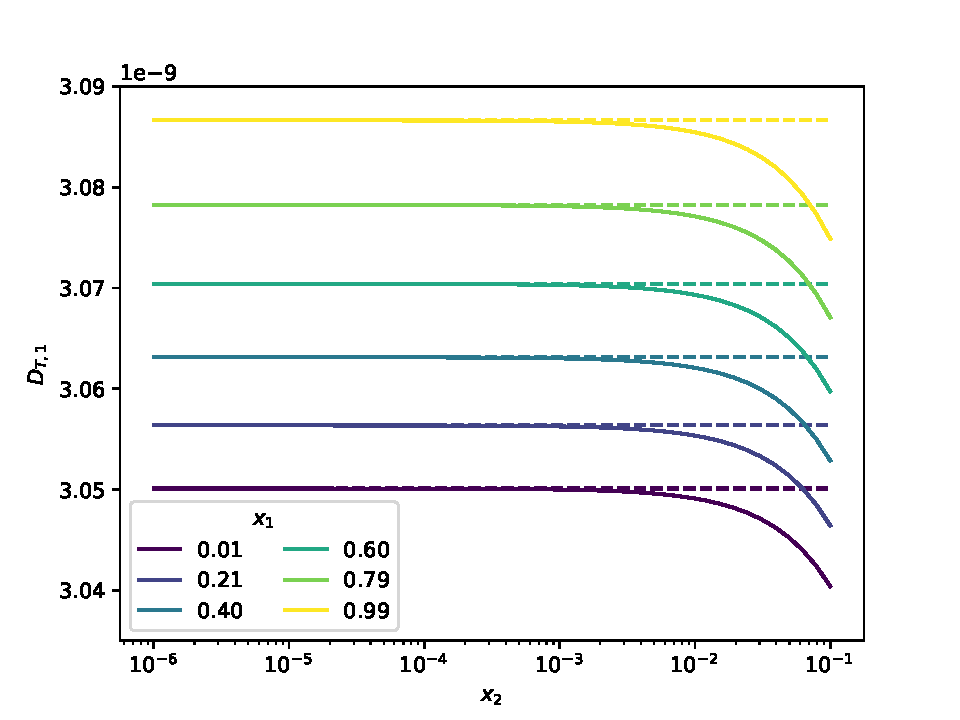
\includegraphics[width=.6\textwidth]{ternary_DT.pdf}
    \caption{The thermal diffusion coefficient $D_{T,1}^{(z, t)}$ in the ternary mixture (1, 2, 3) (solid lines), and the thermal diffusion coefficient $D_{T,1}^{z, b3}$ in the binary mixture (1, 3) (dashed lines), at different mole fractions of species 1 (colors). $x_1$ indicates the mole fraction of species 1 in the binary, i.e. $x_1 = n_1 / (n_1 + n_3)$, such that the composition of the ternary is $\Vec{x}_t = (x_1(1 - x_2), x_2, (1 - x_1)(1 - x_2))$.}
    \label{fig:ternary_DT}
\end{figure}

As seen immediately from Fig. \ref{fig:ternary_DT}, the ternary coefficient (solid lines) approaches the expected binary coefficient as $x_2 \to 0$. Note also the logarithmic scale, and that even at mole fractions of species 2 as small as $x_2 = 10^{-2}$, there is an appreciable difference in $D_{T,1}$ in the ternary compared to the corresponding binary. As seen more clearly in Fig. \ref{fig:ternary_DT_large}, the effect of increasing $x_2$ on $D_{T,1}$ is largest when $x_1$ is large. This could indicate that, contrary to intuition, if one wishes to model a ternary system with $x_1 > x_2 \gg x_3$ as a binary, neglecting the presence of species 3, a better estimate for thermal diffusion is obtained by taking species 2 as the independent species.

Explicitly: For a ternary system consisting of a trace component in air, the best estimate for thermal diffusion appears to be obtained if one models this as a binary mixture of nitrogen with the tracer \textit{taking the tracer to be the independent species}.

\begin{figure}[htb]
    \centering
    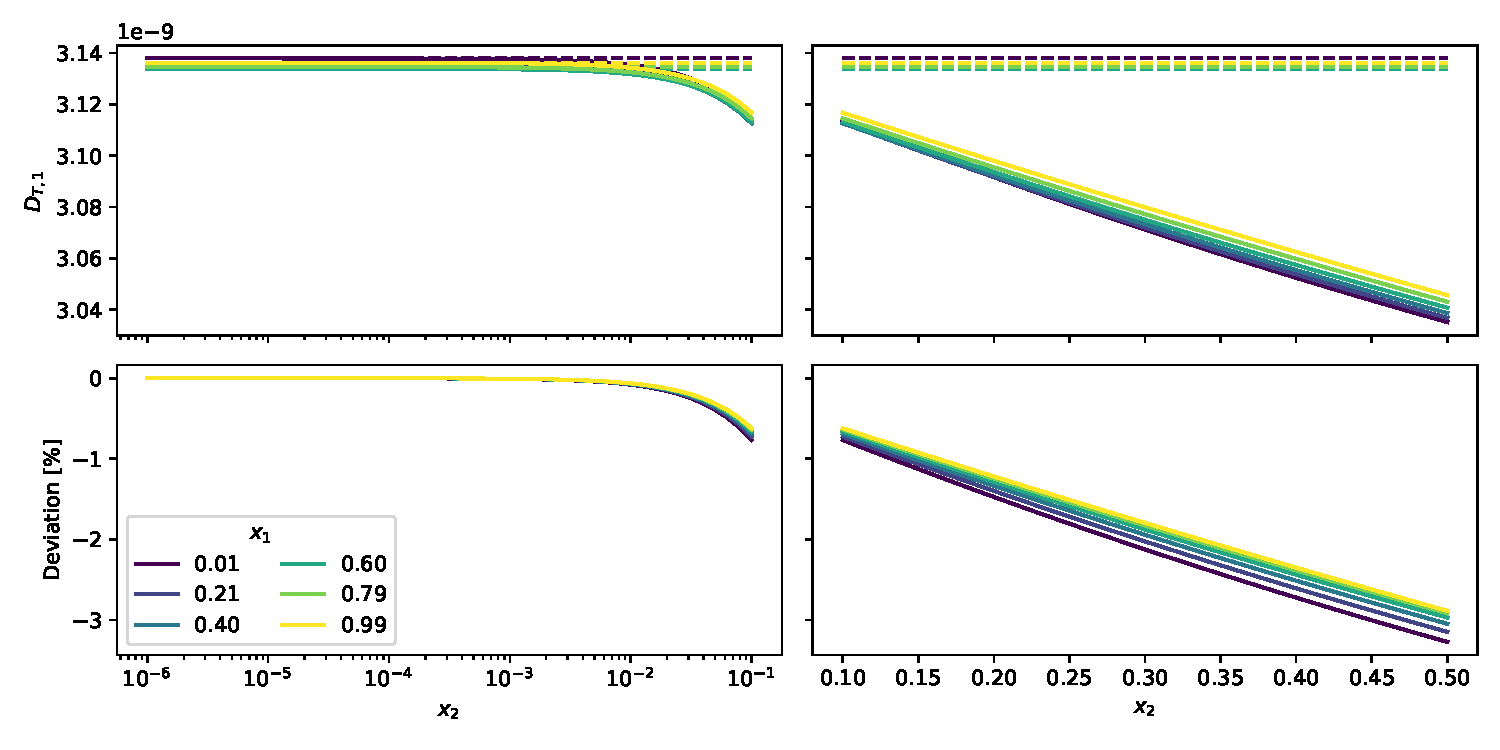
\includegraphics[width=.85\textwidth]{ternary_DT_large.pdf}
    \caption{The same thermal diffusion coefficients as in Fig. \ref{fig:ternary_DT}, with deviations and for a larger composition span.}
    \label{fig:ternary_DT_large}
\end{figure}

\section{Ortiz de Zárate}

Ortiz de Zárate showed that one may define the diffusion- and thermal diffusion coefficients such that they are equivalent in the centre of mass (CoM) and centre of moles (CoN) frame of reference (FoR). We denote these frame-independent coefficients as $\Vec{D}_T^{(z)}$ and $\Mat{D}^{(z)}$, and they are defined through
\begin{equation}
    \begin{pmatrix}J_1 \\ J_2 \\ \vdots \\ J_{N-1} \end{pmatrix}^{(n, n)} = - c\left\{
    \Mat{X}
    \begin{pmatrix}
    D_{T,1} \\ D_{T,2} \\ \vdots \\ D_{T,N-1}    
    \end{pmatrix}^{(z)} \nabla T +
    \Mat{X}
    \begin{bmatrix}
    D_{11} & D_{12} & \hdots & D_{1,N-1} \\
    D_{21} & D_{22} & \hdots & D_{2,N-1} \\
    \vdots & \vdots & \ddots & \vdots \\
    D_{N-1,1} & D_{N-1,2} & \hdots & D_{N-1,N-1}
    \end{bmatrix}^{(z)}
    \Mat{X}^{-1}
    \begin{pmatrix}\nabla x_1 \\ \nabla x_2 \\ \vdots \\ \nabla x_{N-1} \end{pmatrix}
    \right\}
    \label{eq:zarate_definition}
\end{equation}
or, more compactly
\begin{equation}
    \Vec{J}^{(n, n)} = c \left\{ \Mat{X} \Vec{D}_T^{(z)} \nabla T + \Mat{X} \Mat{D}^{(z)} \Mat{X}^{-1} \nabla \Vec{x} \right\},
\end{equation}
where we have arbitrarily chosen the last component as the dependent component for ease of notation, and $\Mat{X}$ is the matrix
\begin{equation}
    X_{ij} = \delta_{ij} x_i - x_i x_j.
\end{equation}
Ortiz de Zárate shows that these coefficients simultaneously fulfill
\begin{equation}
    \Vec{J}^{(m, m)} = \rho \left\{ \Mat{W} \Vec{D}_T^{(z)} \nabla T + \Mat{W} \Mat{D}^{(z)} \Mat{W}^{-1} \nabla \Vec{w} \right\},
\end{equation}
where $w$ denote the mass fractions, $\rho$ denotes the mass density, and $\Mat{W}$ is the matrix
\begin{equation}
    W_{ij} = \delta_{ij} w_i - w_i w_j.
\end{equation}
for details on how these are related to other diffusion coefficients, see the memo on binary limits.

To compute the coefficients $\Vec{D}_T^{(z)}$ and $\Mat{D}^{(z)}$, use the option \code{frame\_of\_reference='zarate'}. For direct access to the coefficients
\begin{equation}
    \begin{split}
        \Mat{D}^{(x)} &= \Mat{X} \Mat{D}^{(z)} \Mat{X}^{-1}, \quad \text{and} \\
        \Mat{D}^{(w)} &= \Mat{W} \Mat{D}^{(z)} \Mat{W}^{-1}
    \end{split}
\end{equation}
use the options \code{frame\_of\_reference='zarate\_x'} and \code{frame\_of\_reference='zarate\_w'}

\clearpage

\bibliographystyle{ieeetr}
\bibliography{bibliografi}

\end{document}
